% ------------------------------------------------------------------------------
% It describes the knowledge about the studied matter through the analysis of
% similar or related published work.
% It provides a comprehensive overview of what was done, what has been done in
% the field and what should be further investigated.
% ------------------------------------------------------------------------------

\opt{never}{\addbibresource{03-tail/bibliography.bib}} % to make citation found in most IDE

\chapter{Analysis}
\label{chap:analysis}

% -- Your text goes here --
The analysis begins by explaining the fundamental concepts that are being worked on throughout the project. Next, a state of the art is provided on the various tools, methods and technologies used in \hyperref[subsec:cloudcomputing]{cloud computing} and \acrshort{iot}.

\minitoc
\newpage

% ------------------------------------------------------------------------------
\section{Definitions}
Before going into more detail on the subject of this work, it is important to look at the definitions of the various terms frequently used.

% -- Your text goes here --
\subsection{Reference architecture}
\label{subsec:ref_arch}
A reference architecture is a solution model in a specific domain. It must be built so that an architecture can be established on its foundations, to make the task of software developers easier.

The aim is to generalise a solution that shows how it works from an overview. It must be possible to observe the relationships and their interactions between the multiple components of the application based on the reference architecture. There are different layers of abstraction depending on the field of application. A high level of abstraction means that it will be possible to understand the solution through more abstract elements such as the general components that will consolidate the application, for example. A low level of abstraction means that the solution will be more precise and certainly more specific to a use case. It will be possible to find detailed relationships between the services contained in the general components.

\subsection{\texorpdfstring{\Gls{cloud}}{} computing}
\label{subsec:cloudcomputing}
The National Institute of Standards and Technology (NIST) \cite{nist_definition_cloud_computing} has standardised the definition of \hyperref[subsec:cloudcomputing]{cloud computing} as follows:
\begin{quote}
    \textit{Cloud computing is a model for enabling ubiquitous, convenient, on-demand network access to a shared pool of configurable computing resources (e.g., networks, servers, storage, applications, and services) that can be rapidly provisioned and released with minimal management effort or service provider interaction. \cite{nist_definition_cloud_computing}}
\end{quote}
It is added in the article \cite{nist_definition_cloud_computing} that this model of \gls{cloud} consists of three service models and four deployment models. The service models are as follows:
\begin{itemize}
    \item[—] \acrfull{iaas} : The capability offered to the consumer consists of providing processing, storage, network and other fundamental computing resources where the consumer can deploy and run arbitrary software, which may include operating systems and applications. The consumer manages the operating systems, storage and applications.
    \item[—] \acrfull{paas} : The capacity provided to the consumer consists of deploying on the \gls{cloud_infrastructure} applications created or acquired by the consumer using programming languages, libraries, services and tools supported by the provider. The consumer manages only the applications and storage.
    \item[—] \acrfull{saas} : The consumer has the option of using the supplier's applications running on a \gls{cloud_infrastructure}. The consumer manages nothing of the infrastructure apart from any configuration of the applications.
\end{itemize}
\begin{center}
    \begingroup
    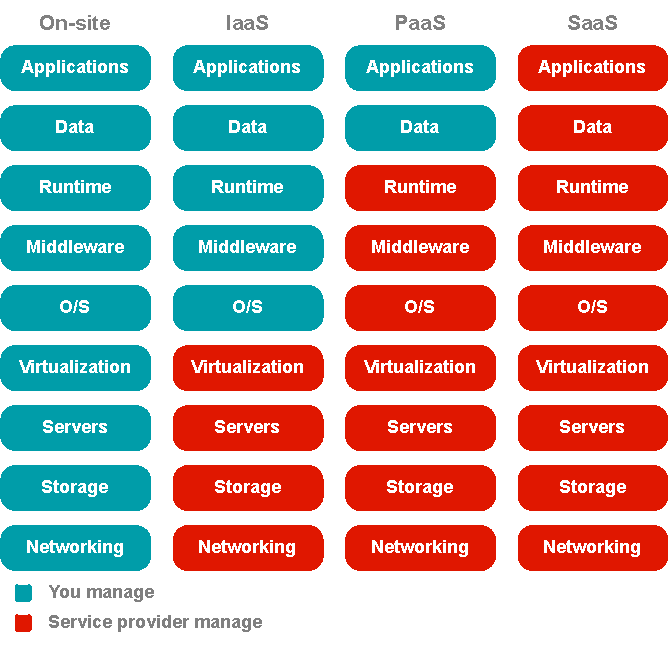
\includegraphics[width=.7\columnwidth]{analysis/iaas_paas_saas.pdf}
    \captionof{figure}{Comparison of different service models \cite{iaas_paas_saas}}
    \label{fig:iaas_paas_saas}
    \endgroup
\end{center}
The deployment models are as follows \cite{nist_definition_cloud_computing} :
\begin{itemize}
    \item[—] \textbf{Private \gls{cloud}} : The \gls{cloud_infrastructure} is made available for exclusive use by a single organisation comprising multiple consumers. It may be owned, managed and operated by the organisation, by a third party or by a combination of both, and it may exist on the organisation's premises or off-site.
    \item[—] \textbf{Community \gls{cloud}} : The \gls{cloud_infrastructure} is reserved for the exclusive use of a specific community of consumers from organisations with common concerns. It may be owned, managed and operated by one or more organisations within the community, by a third party or by a combination of such organisations, and it may exist on or off premises.
    \item[—] \textbf{Public \gls{cloud}} : The \gls{cloud_infrastructure} is made available to the general public for open use. It may be owned, managed and operated by a business, educational institution or government organisation, or a combination of these. It is located on the provider's premises.
    \item[—] \textbf{Hybrid \gls{cloud}} : The \gls{cloud_infrastructure} is a composition of two or more distinct infrastructures (private, community or public) which remain unique entities, but which are linked by a standardised or proprietary technology that allows the portability of data and applications.
\end{itemize}

\subsection{\Gls{cloud}-Native}
\label{subsec:cloudnative}
\nameref{subsec:cloudnative} is an approach to software development which aims to design, implement and manage applications in the \gls{cloud}. \nameref{subsec:cloudcomputing} environments will be necessary for the proper execution of workloads.

The infrastructure can be deployed in private, public or hybrid \glspl{cloud}. This approach will enable the development of modern, easily scalable applications. The flexibility aspect is also emphasised thanks to techniques for decoupling the multiple services of an application. Another strength of the \gls{cloud} is its reliability and sustainability. Since the number of resources is incalculable and they are distributed around the world, redundancy guarantees security in the event of an incident, with almost instantaneous migration of an application's execution. The customer is therefore very often spared any unforeseen events. It is also possible to provide updates in real time and on a recurring basis.

The main benefits are high efficiency, reduced costs and high availability. Applications will be able to exploit resources that are optimal for their use case. The term pay-as-you-go is widely used, as the cost will depend solely on the use made of the resources and not on anything else, such as their maintenance, hardware security, etc. Availability is high because of the astronomical number of resources made available by the various \gls{cloud} environment providers.

\subsection{\acrlong{iot}}
\label{subsec:iot}
\acrfull{iot} refers to the interconnection between physical objects and the internet. Objects can range from light bulbs to medical devices and much more. The main areas concerned are home automation and medical technology.

This involves linking different objects and applications to move into an automated world. As this becomes more and more widespread, the services needed to make it work need a huge amount of resources. This has been made possible by the \gls{cloud}. Everything must be accessible from anywhere in the world, quickly and securely. Several communication technologies are possible to guarantee excellent accessibility and reliability.

% ------------------------------------------------------------------------------
\section{Problem formulation}

% -- Your text goes here --
The general question for analysis is: "Which technologies should be used to develop a reference architecture".

To help answer this question, it is important to consider the following aspects:
\begin{itemize}
    \item[—] Technology
    \item[—] Environment
    \item[—] Tools
    \item[—] Certification
\end{itemize}
Since the development uses the \nameref{subsec:cloudnative} approach, its history can be described first. The integration of the \acrshort{iot} world into \hyperref[subsec:cloudcomputing]{cloud computing} must then be observed through various scientific works and research. A study of \gls{cloud} service providers must be undertaken to differentiate the iot services offered by each one. As the reference architecture is based on an \acrfull{iac}, research into \acrshort{iac} tools is carried out. Finally, it is worth finding out whether SystemReady certification exists for electronic boards using an \gls{arm} processor architecture.


% ------------------------------------------------------------------------------
\section{Literature search}

% -- Your text goes here --
Literature search has focused on academic search engines. The following search engines were used :
\begin{itemize}
    \item[—] \href{https://scholar.google.com}{Google Scholar}
    \item[—] \href{https://ieeexplore.ieee.org/Xplore/home.jsp}{IEEE Xplore}
    \item[—] \href{https://www.sciencedirect.com}{ScienceDirect}
\end{itemize}
The sources were mainly conference papers. Some information was found on websites. The following keywords were used to find sources that met the requirements of this analysis:
\begin{itemize}
    \item[—] integration
    \item[—] embedded systems
    \item[—] \acrshort{iot}
    \item[—] \nameref{subsec:cloudnative}
    \item[—] \gls{cloud}
    \item[—] \hyperref[subsec:cloudcomputing]{cloud computing}
    \item[—] \gls{cloud} providers
    \item[—] \gls{cloud} platforms
    \item[—] \acrlong{iac}
    \item[—] \acrshort{iac} tools
    \item[—] \gls{arm} SystemReady
\end{itemize}


% ------------------------------------------------------------------------------
\section{History of the \texorpdfstring{\nameref{subsec:cloudnative}}{} approach}

% -- Your text goes here --
\nameref{subsec:cloudnative} is a term that has been around for several years. Figure \ref{fig:google_trend_cloud} shows the evolution of this term since 2006. The boom took place around 2016. It is undoubtedly due to the birth of Docker (2013) \cite{docker} and Kubernetes (2014) \cite{k8s}. In 2015, the Cloud Native Computing Foundation \cite{cncf} was created with the aim of making the \nameref{subsec:cloudnative} approach ubiquitous \cite{cncf_charter}.
\begin{center}
    \begingroup
    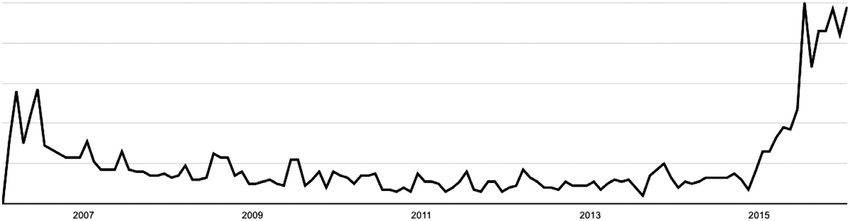
\includegraphics[width=1\columnwidth]{analysis/google_trend_cloud-native.png}
    \captionof{figure}{Google trends (01.01.2006 until 22.05.2016) of term \nameref{subsec:cloudnative} \cite{understanding_cloud_native}}
    \label{fig:google_trend_cloud}
    \endgroup
\end{center}
Before all this, there were only on-site data centres. Generally speaking, each company had its own servers running in its own data centre. This meant that servers were always set up for a specific application. \cite{history_cloud_native}

\subsection{The virtualisation}
The first change came in the 2000s with the virtualisation of servers, although this has been around since the 1960s. When a new application had to be developed, new physical servers had to be bought. With virtualisation, it is no longer necessary to buy new ones. It is possible to run several applications on the same server using virtualisation, which limits the hardware resources for each application (figure \ref{fig:virtualisation}). \cite{history_cloud_native}
\begin{center}
    \begingroup
    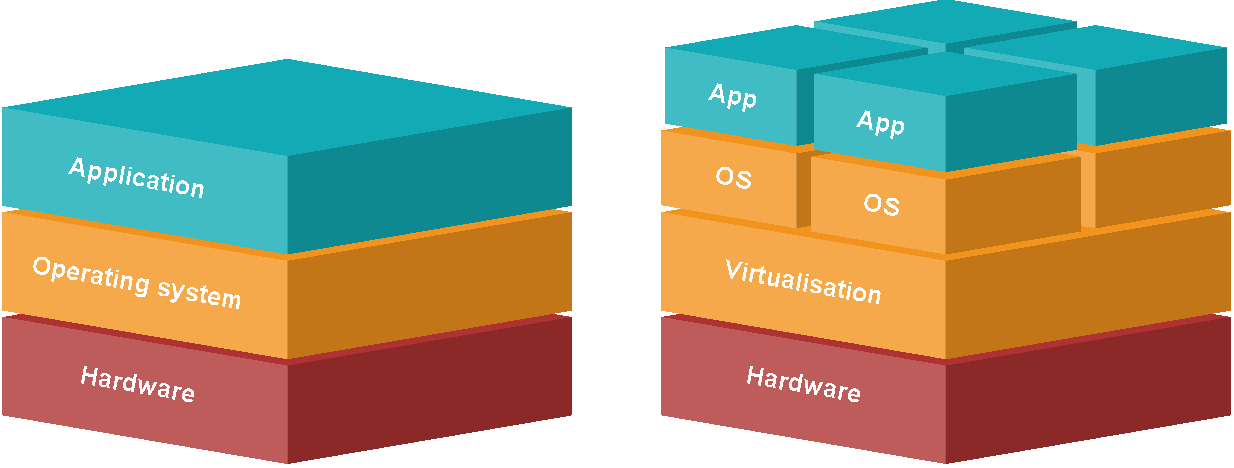
\includegraphics[width=1\columnwidth]{analysis/virtualisation.pdf}
    \captionof{figure}{Traditional server (left) and virtualisation (right)}
    \label{fig:virtualisation}
    \endgroup
\end{center}

\subsection{The hybrid}
Despite this, a minimum of one server had to be purchased for an application to work. There were also resource limits for a certain number of applications. Unfortunately, not everyone could afford to buy new servers. In 2006, \gls{aws} launched three web services, \acrfull{ec2}, Simple Storage Service (S3) and Simple Queue Service (SQS), to allow organisations and individuals to use Amazon's IT infrastructure on an as-needed basis at basic prices \cite{evaluation_aws_services}. This initiative stems from a restructuring of the Amazon platform for better scalability and this has made it possible to sell virtual servers as a service \cite{ec2_origins}. By extension, the myth of making money from servers not in use for the majority of the year has been debunked by Benjamin Black, co-founder of the \acrshort{ec2} \cite{ec2_origins}. This is where the world of \gls{cloud} really began. Kratzke and Quint confirm this in their scientific article \cite{understanding_cloud_native}. The purpose of the \acrshort{ec2} service, which is still used today, is to offer a virtual machine in the \gls{cloud}. This is a \hyperref[subsec:cloudcomputing]{cloud computing} environment for running workloads. It is now possible to migrate your infrastructure from the database to the \gls{cloud}. The corresponding expression is "Lift and Shift" \cite{ibm_lifAndShift}. These were undoubtedly the first so-called \nameref{subsec:cloudnative} approaches \cite{history_cloud_native}. However, this term only appeared in papers for the first time in 2012 \cite{understanding_cloud_native}. These were two conference papers proposing solutions for \nameref{subsec:cloudnative} applications \cite{closer12, 4caast}. Organisations have learned a lot about only paying for what you use. From there, there's a move to hybrid where companies are still using their on-premises servers alongside servers in the \gls{cloud}. \cite{history_cloud_native}

\subsection{All to the \texorpdfstring{\gls{cloud}}{}}
A new barrier has now been crossed. It's no longer a question of doing hybrid, but of transferring the entire infrastructure to the \gls{cloud}. This was made possible when \gls{cloud} service providers such as \gls{aws}, Microsoft Azure, Google Cloud and many others developed several services for all types of use. The reason there are different services is quite simply to decouple application functionality as much as possible. This is known as a microservices architecture. The risk of an entire application being interrupted in the event of a problem is much less likely. However, some organisations still have applications that are several decades old and have a monolithic architecture. It is not necessarily possible to decouple functionalities. That's why they work on a hybrid basis. \cite{history_cloud_native}

\subsection{The \texorpdfstring{\nameref{subsec:cloudnative}}{} approach}
If we ask several engineers today about the definition of the \nameref{subsec:cloudnative} approach, we will find varying interpretations. There are currently three main schools of thought on this subject \cite{history_cloud_native}. The first group considers that an approach is \nameref{subsec:cloudnative} when all the workloads run in the \gls{cloud}. A minority within this group argue that you can be partially \nameref{subsec:cloudnative}, i.e. have one complete application deployed in the \gls{cloud} while maintaining another application locally. However, others feel that this is still a hybrid approach. A second group says that to be truly \nameref{subsec:cloudnative}, you need to fully exploit the capabilities offered by the \gls{cloud}. This means not only using the basic services of a \gls{cloud} provider, but also making full use of the advanced features on offer, such as serverless functions. Some even consider that a company has to be born in the \gls{cloud} to be truly \nameref{subsec:cloudnative}, a phenomenon that is increasingly being observed, with companies launching their first applications directly in the \gls{cloud} without ever having used on-premises servers. This is the case for the company \nameref{subsec:56k.cloud} \colorbox{red}{To be confirmed}. \cite{history_cloud_native}

In 2018, a brief history of \gls{cloud} application architectures described the term \nameref{subsec:cloudnative} as follows :
\begin{quote}
    \textit{\Glspl{cloud_infrastructure} (\acrshort{iaas}) and platforms (\acrshort{paas}) are built to be elastic. Elasticity is understood as the degree to which a system adapts to workload changes by provisioning and de-provisioning resources automatically. Without this, \hyperref[subsec:cloudcomputing]{cloud computing} is very often not reasonable from an economic point of view. Over time, system engineers learned to understand this elasticity options of modern \gls{cloud} environments better. Eventually, systems were designed for such elastic \glspl{cloud_infrastructure}, which increased the utilization rates of underlying computing infrastructures via new deployment and design approaches like containers, microservices or serverless architectures. This design intention is often expressed using the term \nameref{subsec:cloudnative}. \cite{history_cloud_application}}
\end{quote}


% ------------------------------------------------------------------------------
\section{Integrating \texorpdfstring{\hyperref[subsec:cloudcomputing]{cloud computing}}{} with \texorpdfstring{\acrshort{iot}}{} embedded systems}

% -- Your text goes here --
With technology advancing at a rapid pace, today's world appreciates help in making everyday life better \cite{state_of_the_art_integration_iot_cloudComputing}. Embedded systems that have become increasingly connected now offer this service. However, since they need to attend any location for any domain and task, they need to be small for better integration. As a result, resources are limited for computing operations, data storage, data processing and so on. The built-in security and low energy consumption that these devices must also ensure are not enough to allow them to move forward. This is why \hyperref[subsec:cloudcomputing]{cloud computing} needs to be integrated to fill the gaps left by \acrshort{iot} \cite{state_of_the_art_integration_iot_cloudComputing}. Cloud of Things is one of the paradigms given to the combination of these two technologies in 2014 \cite{cloud_of_thing}.

\subsection{Overview}
A model for integrating \hyperref[subsec:cloudcomputing]{cloud computing} into an embedded system is shown in figure \ref{fig:device_and_cloud_computing}. \cite{integration_embedded_systems_cloudComputing}
\begin{center}
    \begingroup
    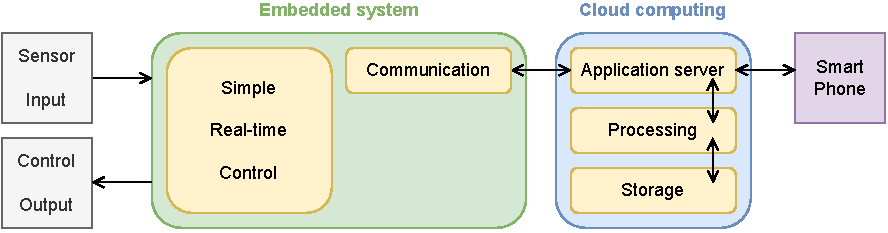
\includegraphics[width=1\columnwidth]{analysis/device_and_cloud_computing.pdf}
    \captionof{figure}{Model for integrating \hyperref[subsec:cloudcomputing]{cloud computing} into an embedded system \cite{integration_embedded_systems_cloudComputing}}
    \label{fig:device_and_cloud_computing}
    \endgroup
\end{center}
The main idea is to use only what is necessary on the \acrshort{iot} device. In other words, all computing and storage functions should be moved to the \gls{cloud}. The device should only be linked to the input and output peripherals using a simple controller and establish communication with the \gls{cloud}. For the integration to work, the embedded system must have an internet connection. \hyperref[subsec:cloudcomputing]{Cloud computing} would contain the core of the application as well as various services to perform analysis, processing and calculation operations, and store data in real time. From there, it would also be possible to view the data from a smartphone. This approach is a solution that was thought up by Furuichi and Yamada in 2014 \cite{next_generation_iot_cloud}. It offers a number of advantages, such as reduced energy consumption by eliminating large workloads and reduced size by freeing up electronic components. The \gls{cloud} also makes it easy to scale up if necessary. The application can then be highly scalable. \cite{integration_embedded_systems_cloudComputing}

Furuichi and Yamada wanted to use a project to prove that their suggested approach worked. They developed a traffic jam detection system that recognises car licence plate numbers along with their location and time. For a plate number to be recognised from a raw image, image processing is carried out using machine learning. They found that this application, split between an \acrshort{iot} device and a \hyperref[subsec:cloudcomputing]{cloud computing} environment, scored much better than the same application managed entirely on a laptop or embedded system. The evaluation looked at cost, battery life, performance, scalability and reliability. \cite{next_generation_iot_cloud}

\subsection{Reference architecture}
A reference architecture has been developed to support \acrshort{iot} objects in \hyperref[subsec:cloudcomputing]{cloud computing} (figure \ref{fig:reference_architecture_CSCC}). The Standards Development Organization has decided to make this a standard by launching the Cloud Standards Customer Council programme to drive forward the adoption of \hyperref[subsec:cloudcomputing]{cloud computing}. In this architecture, various aspects are taken into account: scalability, security, reliability and protection of privacy. \cite{reference_architecture_cloud_iot}
\begin{center}
    \begingroup
    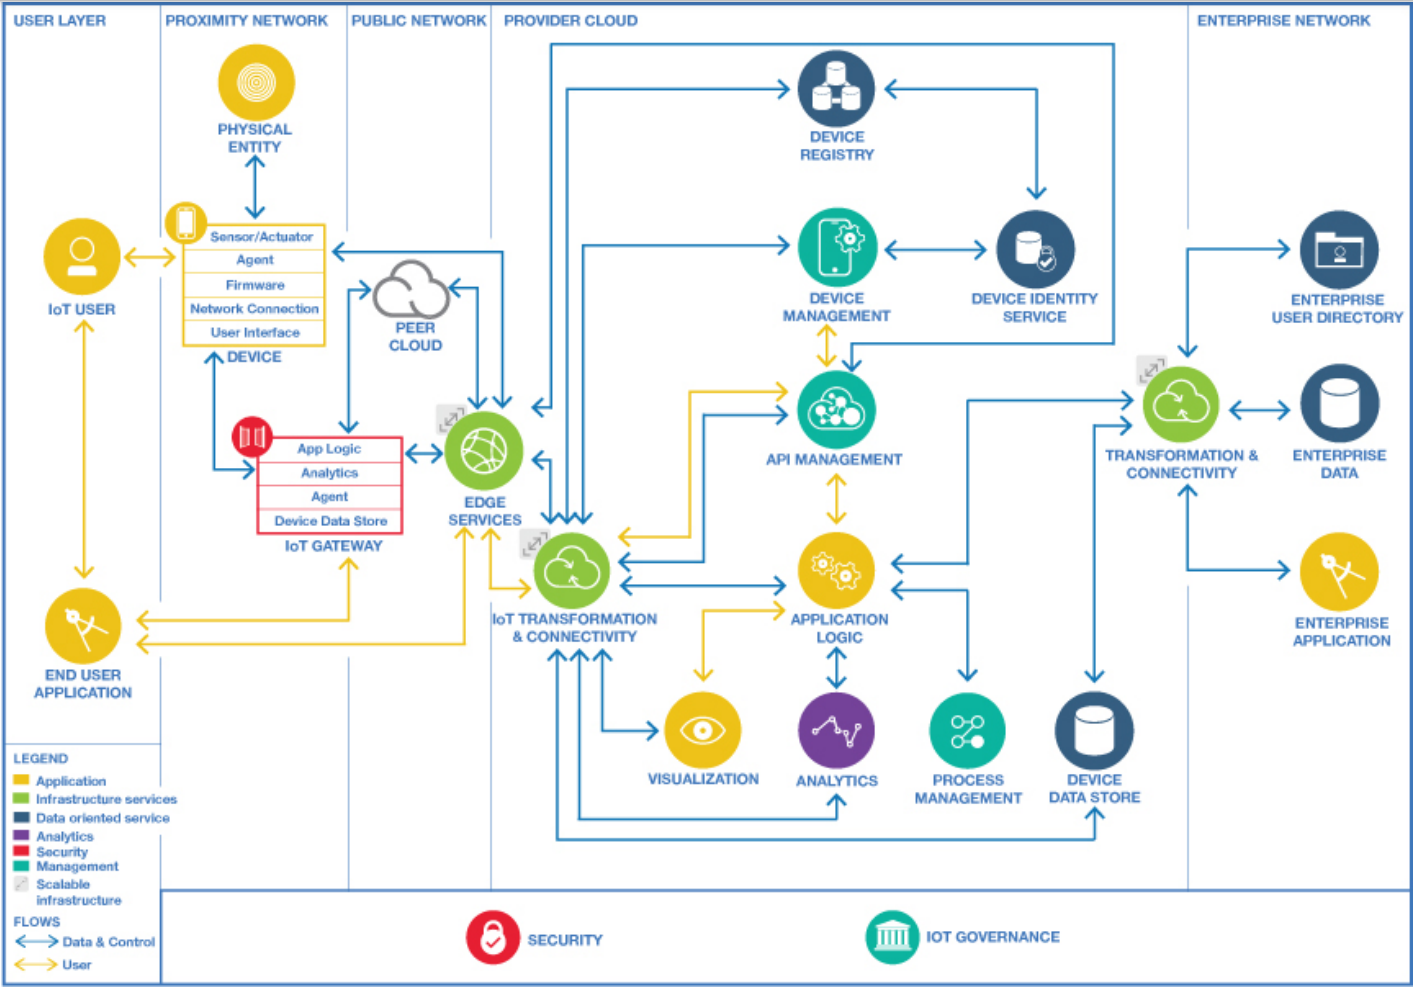
\includegraphics[width=1\columnwidth]{analysis/reference_architecture_CSCC.png}
    \captionof{figure}{Cloud Customer Reference Architecture for IoT \cite{reference_architecture_cloud_iot}}
    \label{fig:reference_architecture_CSCC}
    \endgroup
\end{center}
The architecture proposed in figure \ref{fig:reference_architecture_CSCC} is made up of components and their relationships. They are separated under a three-tier architecture model, called 3-Tier (presentation, logic, data). There is edge-tier, the platform tier and the enterprise tier.

The edge-tier contains the "Proximity Network" and "Public Network" parts. It represents the place where data is collected. It is collected from an \acrshort{iot} device in a proximity network. The data will either be sent to an \acrshort{iot} gateway or directly to the \gls{cloud} provider.

The \gls{cloud} provider tier manages the entire logical part of the application. It includes the collection, processing and analysis of data flows. Each device is also managed in this tier, as is its identity, for example.

The enterprise tier contains the "Enterprise Network" part. It includes the enterprise data and the application. Data from \hyperref[subsec:cloudcomputing]{cloud computing} can be stored in enterprise data.

\subsection{Existing problems and solutions linked to integration}
Integrating \acrshort{iot} and \hyperref[subsec:cloudcomputing]{cloud computing} poses a number of challenges. They are to be found both on the hardware side and in the \gls{cloud}. \cite{cloud_of_thing}

There are many communication protocols. There are protocols for every type of use. On the \acrshort{iot} side, for example, there are Zigbee \cite{zigbee}, Bluetooth and \acrfull{ble} \cite{bluetooth}, LoRaWAN (long range) \cite{lora_alliance}, \acrshort{wifi}, Thread \cite{thread} and the latest Matter protocol \cite{matter}. In an \acrshort{iot} network, there can be a multitude of sensors linked to a gateway. Interoperability is a problem in this case. Since 2022, version 1.0 of the Matter protocol has been published to address this problem. However, few devices are yet compatible. In research projects, Zigbee is very popular \cite{state_of_the_art_integration_iot_cloudComputing, cloud_of_thing, secure_integration_iot_cloud_computing, smart_home_integration}. Two main technologies are used for communication between the \acrshort{iot} gateway and the \gls{cloud}: \acrfull{mqtt} \cite{mqtt} and \acrfull{coap} \cite{coap_whitepaper}. Several projects have used \acrshort{coap} for resource reasons \cite{cloudthings, actinium_integration_solution, aws_arm_architecture_iot}. It is a protocol dedicated to constrained devices with small amounts of memory \cite{coap_whitepaper}, using \acrshort{udp}. It is also suitable for devices that need to bind to web services as it uses the \acrfull{rest} model. \acrshort{rest} is an architectural style for web services \cite{cloudthings}. It would have been possible to use the \acrfull{soa} style, but it is less suited to this use case \cite{cloudthings}. Service-based architecture styles allow a high degree of decoupling from the application. This is an advantage in the event of a problem with a service, so as not to completely freeze the application. Finally, \acrshort{mqtt} is specially designed for \acrshort{iot} \cite{mqtt}. It uses the \acrshort{tcp} transport protocol. \Gls{cloud} provider \gls{aws} adopts the \acrshort{mqtt} protocol in its \acrshort{iot} sector \cite{mqtt_aws}. A communication between an \gls{arm} microcontroller and \gls{aws} proved that this protocol works \cite{aws_arm_architecture_iot}. In fact, the data passing through is often in \acrfull{json} format \cite{integration_embedded_systems_cloudComputing, smart_home_integration, itaas_reference_architecture}. This is a lightweight data representation syntax for storing and exchanging textual information \cite{smart_home_integration}. There is also the \acrfull{http} communication protocol. It would be suitable for updating \acrshort{iot} devices. It allows more bytes to be sent per packet, which increases the update speed. Furthermore, in industry, \acrshort{http} is generally less constrained by firewalls than \acrshort{mqtt} or \acrshort{coap} \cite{OTA_Solution_proposed}.

A lot of energy is consumed in \acrshort{iot} devices. The reason for this is the increasing amount of data being transferred to the \gls{cloud}. Energy needs to be managed efficiently, for example by setting a sleep mode. If this is not possible, natural energy could be used to provide power, such as solar, wind or vibration. \cite{cloud_of_thing}

Resource allocation is another debate. Each \acrshort{iot} object may have a different function. They do not necessarily require the same resources in the \gls{cloud}. What's more, unexpected events could occur requiring a greater workload. The requirements could not necessarily be predictable. Even if they were, the cost of increasing unused resources for most of the time would be a loss. \Gls{cloud} service providers offer a number of solutions to this problem. For example, \gls{aws} offers a service that balances the load in the \hyperref[subsec:cloudcomputing]{cloud computing} environment \cite{elb_aws}. The combinatorial auction approach is popular for resource allocation in the \gls{cloud} \cite{optimization_resources_allocation}. It must satisfy \acrfull{qos} constraints and maximise the \gls{cloud} provider's profit. Provider and user profit, resource utilisation and quality of service are the dominant performance factors. Research has succeeded in optimising this approach \cite{optimization_resources_allocation}. Nevertheless, as soon as a new \acrshort{iot} node is added, a sample of data could be sent to the \gls{cloud} to set up the minimum resources required. \cite{cloud_of_thing}

Identity management in an internet network is very important to ensure that each device is unique. Given the number of \acrshort{iot} devices today, IPv6 addressing would be the optimal solution. It would be sufficient to support this type of network. However, deployment remains problematic. The coexistence of IPv6 with IPv4 is not so easy \cite{cloud_of_thing}. There are three possible techniques for cooperation between the two \cite{coexistence_ipv4_ipv6}. The \acrshort{iot} device may support both types of addressing. Alternatively, IPv6 packets must be encapsulated in IPv4 packets, or a \acrfull{nat} must be available that translates both types of packet.

The discovery of new \acrshort{iot} devices to be integrated into the \gls{cloud} needs to be managed. At any time, a device can be part of a service and leave it. It is also necessary to monitor its status once it is connected and keep it up to date. \gls{aws} enables a component to be deployed on \acrshort{iot} devices that links to the \gls{cloud}. From there, it is possible to perform \acrfull{ota} updates \cite{ota_aws_iot} and monitor the state of the device \cite{status_aws_iot}. Azure also provides these different services \cite{ota_azure_iot, status_azure_iot}. An update method was designed in this area in 2022 \cite{OTA_Solution_proposed}. It is based on the standard update architecture for \acrshort{iot} \cite{firmware_update_architecture_iot}, proposed by the Internet Engineering Task Force (IETF).

\hyperref[subsec:cloudcomputing]{Cloud computing} environments must respond correctly to data flows, whether large or small. The urgency with which certain data is transmitted is also an integral part of this \acrshort{qos}. \acrshort{qos} is assessed in terms of bandwidth, delay, packet loss rate and delay in the transmission of data packets (jitter). \cite{cloud_of_thing}

Another point to consider is where the data is stored. Depending on the volume of data, it is best to store it in the physical location closest to the user. Sensitive data must also be managed in accordance with each country's data protection laws. Fortunately, \gls{cloud} providers offer the option of choosing the region where data is stored. \cite{cloud_of_thing}

Security seems to be an issue in integration. In 2016, there was a lack of trust in \gls{cloud} service providers and a lack of awareness of Service-Level Agreements (SLAs) \cite{survey_integration_iot_cloud_computing}. A Service-Level Agreement is a document defining the provision of \gls{cloud} services and the responsibilities of the provider and the customer. \nameref{subsec:56k.cloud} claims some negligence with developers. However, when data is transferred to the \gls{cloud}, the location of databases is not always transparent. Distributing data over several locations, while ensuring high availability, also increases the chances of sensitive data being leaked. A distributed system of this kind is exposed to various potential attacks, such as SQL injections, cross-site scripting attacks and many others. Significant vulnerabilities can also be exposed, including session hijacking and virtual machine evasion. In addition, the computing power constraints associated with connected objects limit the application of public key cryptography to all layers of the system. Two years later, in 2018, in an attempt to partially address this problem, two security models have been proposed using two encryption algorithms (AES and RSA) \cite{secure_integration_iot_cloud_computing}. They can be used to integrate \acrshort{iot} and \hyperref[subsec:cloudcomputing]{cloud computing}. However, they remain sub-optimal and could be the subject of future research.

Unnecessary data communication is a current trend. \acrshort{iot} devices generate all kinds of data. It would be interesting to have an \acrshort{iot} gateway that manages traffic by letting data circulate only when it is necessary and only that which is necessary \cite{cloud_of_thing}. This would save energy and make better use of network and \gls{cloud} resources. An architecture for this approach has been presented \cite{unnecessary_data_architecture}.


% ------------------------------------------------------------------------------
\section{\texorpdfstring{\acrshort{iot}}{} \texorpdfstring{\gls{cloud}}{} platforms}
\label{subsec:cloud_providers}

% -- Your text goes here --
A number of projects have created their own \gls{cloud} platform \cite{Ilyas_Ahmad_Saleem_2020}. The University of Glasgow decided to create its own \hyperref[subsec:cloudcomputing]{cloud computing} environment based on a Raspberry Pi \cite{raspberrypi}, called PiCloud \cite{glasgow_rpi_cloud_computing}. It emulates every layer of a \gls{cloud} stack, from resource virtualisation to network behaviour. A fleet of 56 Raspberry Pi devices was able to consolidate this \gls{cloud} platform. This project is ideal for education, thanks to its low cost. Another study, based on the previous one, carried out the same style of \gls{cloud} platform, but with 300 Raspberry Pi devices. Called the Bolzano Raspberry Pi \cite{bolzano_rpi_cloud_computing}, this \hyperref[subsec:cloudcomputing]{cloud computing} environment incorporates several \acrfull{nas} as storage units. However, these are traditional \glspl{cloud_infrastructure}.

\Glspl{cloud_infrastructure} have been adapted for the use of \acrshort{iot}. What differentiates them from traditional infrastructures is the processing of data generated by events in real time \cite{Sikarwar_Yadav_Dubey_2020}. There are now a large number of public \gls{cloud} service providers for \acrshort{iot}. There are also a number of open source \acrshort{iot} solution providers. The main ones today are \gls{aws}, Microsoft Azure and Google Cloud \cite{gartner_cloud_providers_ranking}.

\gls{aws} \cite{amazon_web_services} provides a \gls{cloud} platform with over 200 services. Resources are distributed across 32 regions worldwide. It claims to be the most widely adopted platform in the world. Products include: compute, storage, databases, analytics, networking, mobile, development tools, management tools, \acrshort{iot}, security and enterprise applications. It offers its services on demand and payment is on a pay-as-you-go basis. Through a survey published in 2019 on the various platforms \cite{survey_iot_platform_comparison}, a solution dedicated to \acrshort{iot}, called \gls{aws} \acrshort{iot}, was summarised. This service aims to collect, store and analyse data from devices. Amazon FreeRTOS and \gls{aws} \acrshort{iot} Greengrass are made available by \gls{aws} \acrshort{iot}, facilitating the development of embedded applications on these devices. For embedded systems, both \gls{arm} and x86 architectures with Linux are supported \cite{fog_computing_platforms_comparison}. For device management, there is \gls{aws} \acrshort{iot} Core, which facilitates device connectivity with \gls{cloud} services. This can be complemented by \gls{aws} \acrshort{iot} Things Graph to visualise the data emitted by devices. In terms of data processing, the platform provides \gls{aws} \acrshort{iot} Analytics, offering developers a convenient way to analyse the data generated. The results of this process can be routed to other devices or systems via the \gls{aws} \acrshort{iot} Events service \cite{survey_iot_platform_comparison} service. The aim of a thesis project was to define an \acrshort{iot} architecture for connecting \gls{arm} microcontrollers to \gls{aws} \cite{aws_arm_architecture_iot}. An example of a smart home application was made on this architecture. A machine learning service was used in the \hyperref[subsec:cloudcomputing]{cloud computing} to make predictions from data sent from the \acrshort{iot} devices. The company \nameref{subsec:56k.cloud} is also carrying out a few projects linking \gls{arm} devices with a \gls{cloud_infrastructure} \gls{aws}. Typically, it uses the \gls{aws} \acrshort{iot} Greengrass Core component to run applications on embedded systems.

Microsoft Azure \cite{microsoft_azure} is another public \gls{cloud} provider. Launched in 2008, it offers more than 200 \gls{cloud} products and services. Its data centres are located in more than 60 regions around the world. The company operates in the healthcare, finance, public sector, manufacturing and retail sectors. It says it invests a billion dollars a year in security to protect customer data. As far as \acrshort{iot} is concerned, it offers a solution called Azure \acrshort{iot}. This solution includes several services. Azure \acrshort{iot} Hub is a service that establishes connections, administers and develops the ability to manage billions of \acrshort{iot} devices, from the peripheral to the \gls{cloud}. Azure \acrshort{iot} Central provides a user interface and \acrshort{api}s for connecting and managing large-scale embedded systems. Data is visualised using Azure Time Series. Azure Sphere offers security to protect \acrshort{iot} devices. Physical device spaces can be replicated using the Azure Digital Twins service. System logic can be managed by Azure \acrshort{iot} Edge. For the development of integrated applications, there is Azure RTOS. \cite{microsoft_azure}

Google \Gls{cloud} \cite{google_cloud} is one of the world's leading \gls{cloud} providers. It currently distributes its resources in 39 regions across the globe. Launched in 2008, the provider is trying to keep up with the competition by offering around a hundred services for all types of business. However, Google has announced that it will be pulling out of the \acrshort{iot} business in 2023. The Google \Gls{cloud} spokesperson said that the needs of their customers could be better served by specialist \acrshort{iot} partners \cite{akenza_google_cloud_iot}.

There are other \gls{cloud} providers offering \acrshort{iot} services. Some of these are mentioned in figure \ref{fig:cloud_providers}, where a comparison is made.
\begin{center}
    \begingroup
    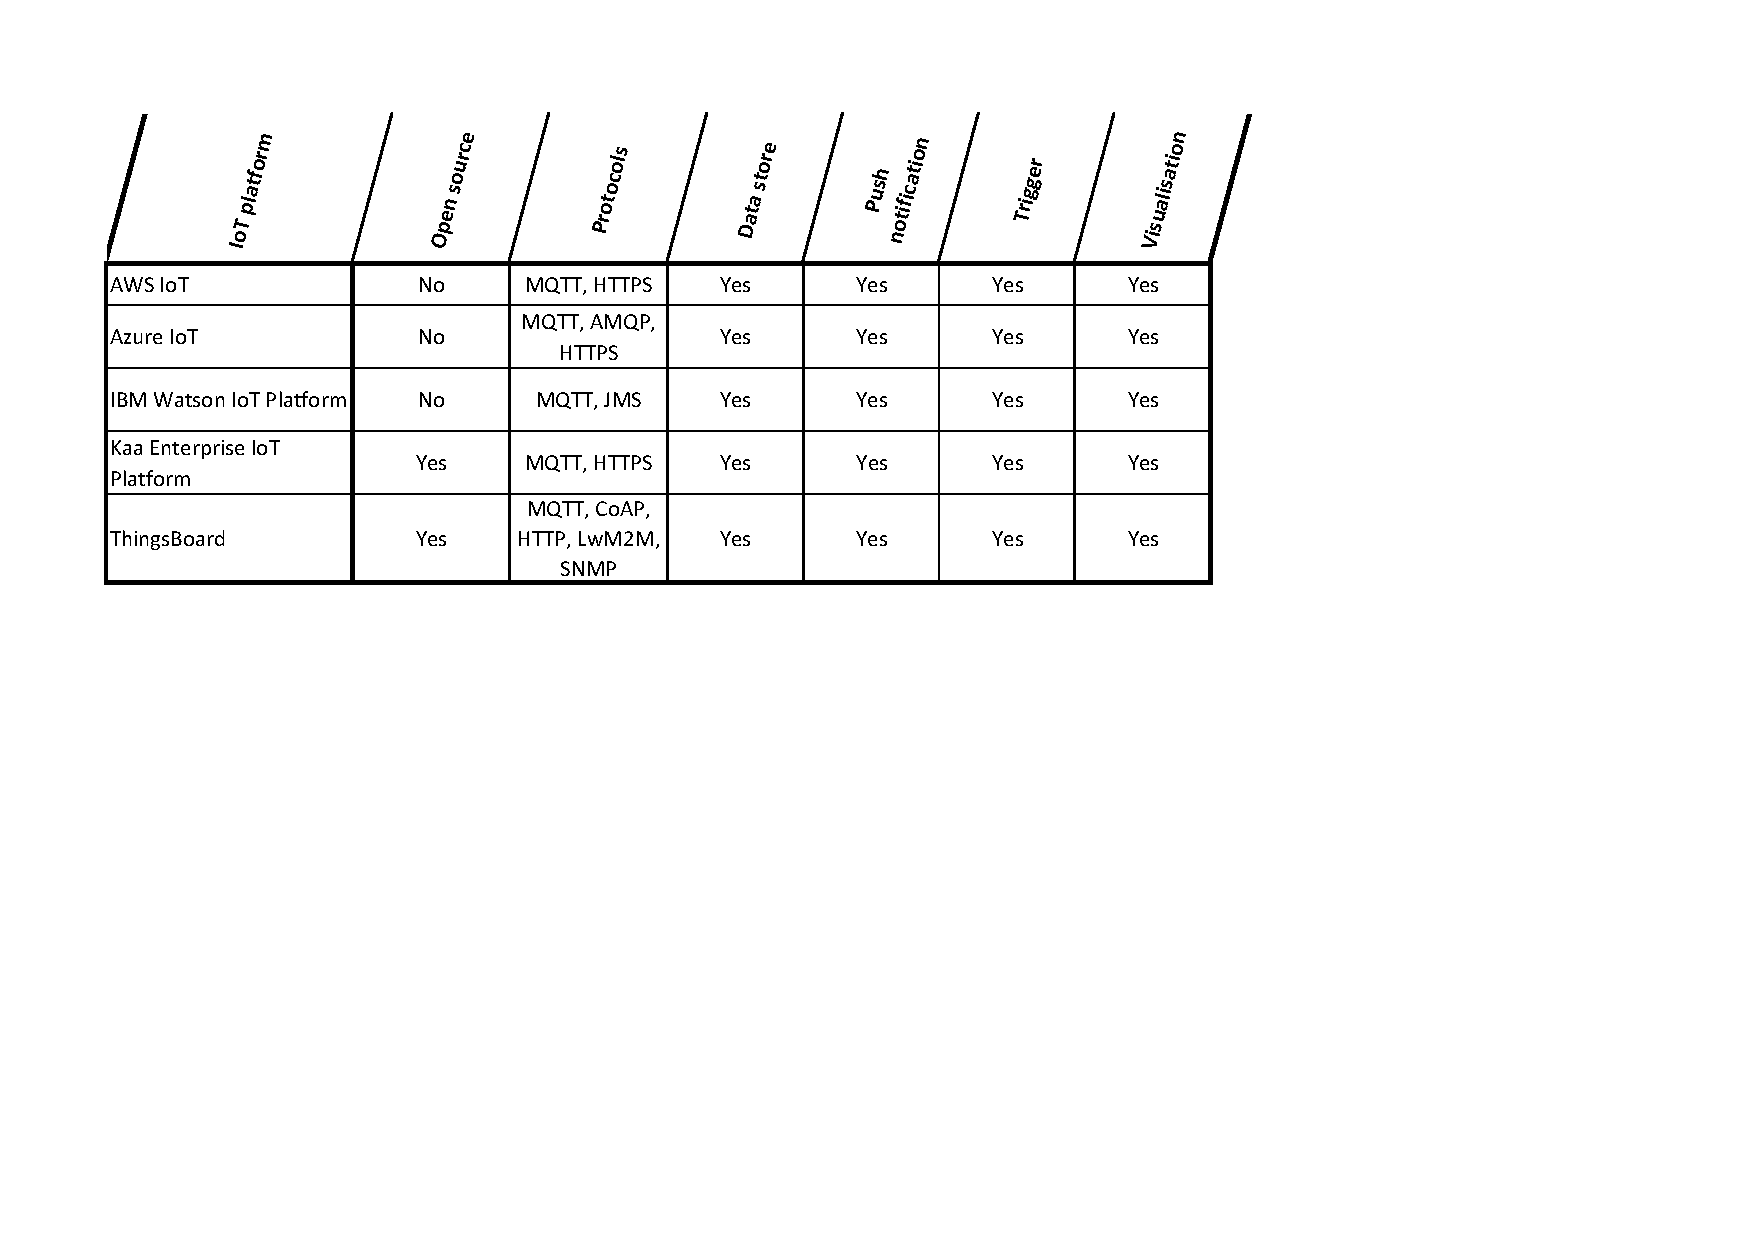
\includegraphics[width=1\columnwidth]{analysis/cloud_providers.pdf}
    \captionof{figure}{Comparison of \acrshort{iot} \gls{cloud} platform providers (sources from providers)}
    \label{fig:cloud_providers}
    \endgroup
\end{center}
Looking at the back end of platforms, they would have an advantage in using containerisation over traditional virtual machines \cite{container_cloud_platform}. It is seen as a lightweight virtualisation solution, with greater flexibility. In addition, containers are proving particularly suitable for solving the platform issues commonly associated with \acrshort{paas} services in the \gls{cloud}. This includes aspects such as application packaging and coordination \cite{container_cloud_platform}. Docker is the most popular container solution \cite{docker}. As for container orchestration, there's Kubernetes, an open source system \cite{k8s}.


% ------------------------------------------------------------------------------
\section{\texorpdfstring{\Gls{cloud}}{} infrastructure tools}
\label{subsec:iac_tools}

% -- Your text goes here --
When you want to host applications in the \gls{cloud}, you need to deploy a \gls{cloud_infrastructure}. It is perfectly possible to build the infrastructure manually. All you have to do is visit a \gls{cloud} provider's web page and select the resources you need from the services on offer. However, this infrastructure could be deployed several times. Fortunately, there are tools that can automatically deploy \glspl{cloud_infrastructure}, called \acrfull{iac}. The automatic deployment of \glspl{cloud_infrastructure} corresponds to \gls{provisioning}. These tools use templates containing a description of the infrastructure based on executable code or a configuration file. They save time on deployment and ensure that the implementation policy behind the infrastructure is always the same (security, rules, etc.). In addition to \gls{provisioning}, \acrshort{iac} tools are capable of updating and deleting an infrastructure. There are universal \gls{provisioning} tools for different \gls{cloud} providers and there are integrated tools for each provider. \cite{iac_tools}

\subsection{Integrated \acrshort{iac} tools}
Having mentioned the \gls{aws} and Microsoft Azure providers in section \ref{subsec:cloud_providers}, each of them has its own \acrshort{iac} tool reserved for use with its platform. Google \Gls{cloud} is not mentioned in this section due to the cessation of \acrshort{iot} activities.

At \gls{aws}, there are two \acrshort{iac} tools. \gls{aws} CloudFormation \cite{aws_cloudformation} is the first. \gls{aws} \acrfull{cdk} \cite{aws_cdk} is the second for defining and building infrastructure in the \gls{aws} \gls{cloud} environment. \gls{aws} \acrshort{cdk} gives users the flexibility to define infrastructure in distinct programming languages in the form of an application, with imperative syntax. It uses \gls{aws} CloudFormation as the deployment engine and allows users to define the infrastructure using programming idioms to model the system design. The \acrshort{cdk} application deployment process includes the construction of the defined elements, preparation, validation and synthesis of the deployment artefacts. The \acrshort{cdk} application is then transferred to the \gls{aws} CloudFormation service for real deployment. An overview of the deployment is shown in figure \ref{fig:aws_iac}. The basic elements of \acrshort{cdk} applications are called "constructs", and they represent \gls{cloud} components containing services. Constructs can be nested to create a hierarchy of dependencies called a "construct tree". Ultimately, this hierarchy defines how constructs are synthesized into resources in the final \gls{aws} CloudFormation model. In a \acrshort{cdk} application, it is possible to define several stacks. These are unique deployment units, each containing a hierarchy of constructs. \cite{iac_tools}
\begin{center}
    \begingroup
    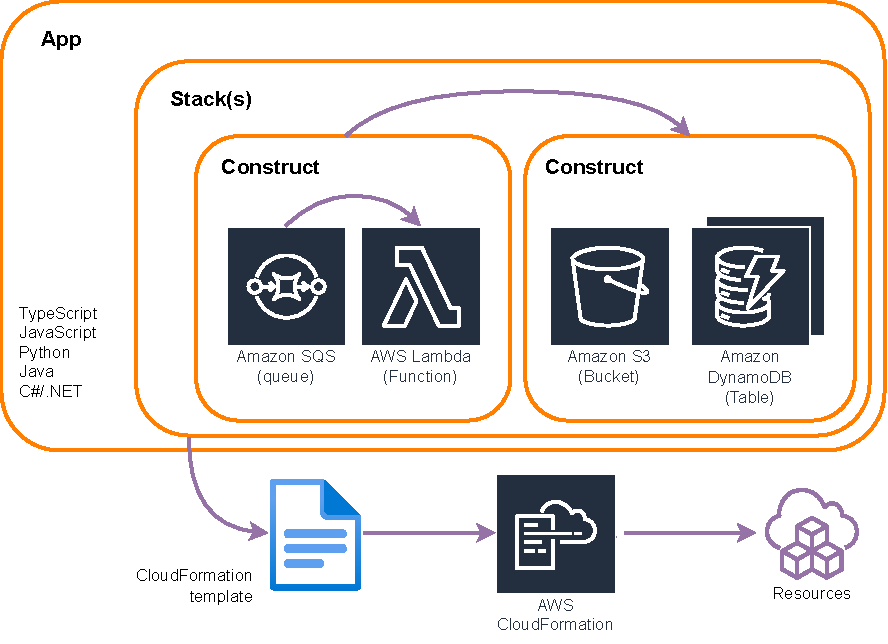
\includegraphics[width=1\columnwidth]{analysis/aws_iac.pdf}
    \captionof{figure}{Overview of \gls{aws} \acrshort{cdk} \cite{aws_cdk} deployment \cite{aws_cdk}}
    \label{fig:aws_iac}
    \endgroup
\end{center}

Microsoft Azure offers the \acrfull{a_arm} deployment and management service \cite{azure_arm}. All actions performed on resources by the user go through the \acrshort{a_arm} manager. It authenticates and authorises them. At the deployment level, there are \acrshort{a_arm} models, which are \acrshort{json} files defining the infrastructure and configuration of a \gls{cloud} environment. \acrshort{json} uses declarative syntax. Before deployment, the \acrshort{a_arm} \acrshort{api} checks the models for possible errors, guaranteeing successful deployment. \acrshort{a_arm} models ensure an identical architecture for deployments in different environments, such as development, testing and production, for example. The fewer dependencies there are, the faster \acrshort{a_arm} can deploy infrastructure resources in parallel. \acrshort{a_arm} models can be segmented into modular files for easy reuse. A group of resources deployed in the Azure platform can be extracted in the form of an \acrshort{a_arm} model. \cite{iac_tools}

\subsection{Universal \acrshort{iac} tools}
There are several \acrshort{iac} tools compatible with different \gls{cloud} platforms such as \gls{aws}, Microsoft Azure, and many others. The \nameref{subsec:56k.cloud} company mainly uses Terraform \cite{terraform} and Pulumi \cite{pulumi}.

Terraform is a tool created in 2014 by HashiCorp, written in the Go programming language \cite{terraform_github}. It mainly provisions \acrlong{iaas}, but can also deploy \acrlong{paas} and \acrlong{saas}. Terraform works using two inputs: configuration and state. The desired resources in the \gls{cloud_infrastructure} are described in a configuration file. This file works with the Terraform language using declarative syntax. The state corresponds to the current state of the infrastructure, or in other words the stack. The state is managed by the Terraform \acrshort{api} and is stored locally by default. The deployment engine compares the desired infrastructure with the current state and determines which resources need to be created, updated or deleted. Terraform uses provider plugins to interact with \gls{cloud} providers. It offers five basic commands for different stages: "init", "validate", "plan", "apply" and "destroy", enabling the infrastructure to be managed efficiently and easily \cite{terraform}. The "init" command prepares the project directory. The "validate" command checks that the configuration is valid. The "plan" command displays the changes required by the current configuration. The "apply" command creates or updates the \gls{cloud_infrastructure}. Finally, the "destroy" command destroys the \gls{cloud_infrastructure}. An overview of the deployment can be seen in figure \ref{fig:terraform_iac}. \cite{iac_tools}
\begin{center}
    \begingroup
    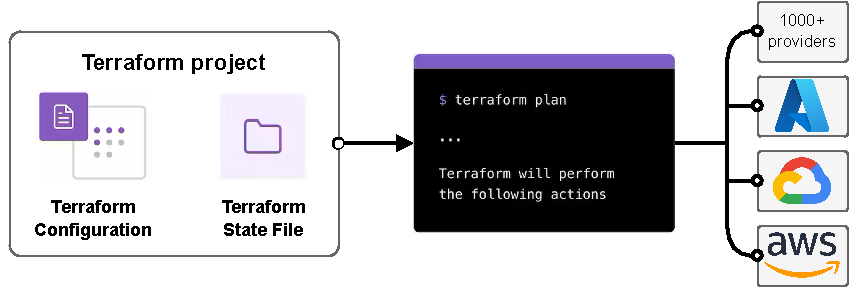
\includegraphics[width=1\columnwidth]{analysis/terraform_iac.pdf}
    \captionof{figure}{Overview of Terraform deployment \cite{terraform}}
    \label{fig:terraform_iac}
    \endgroup
\end{center}

Pulumi is an \acrshort{iac} tool similar to Terraform, but open source. It is written in the Go language \cite{pulumi_github}. Version 1.0 of Pulumi was released in 2019. This tool can be used with several programming languages, such as TypeScript, JavaScript, Python, Go and .NET. It therefore offers developers the possibility of creating \glspl{cloud_infrastructure} using standard technologies, unlike Terraform. Deployment follows the Terraform model, where a Pulumi application is run to schedule the desired resources in the \gls{cloud_infrastructure}. The deployment engine compares these desired resources with the current state of the stack and determines the necessary actions. The state of the last infrastructure deployment is saved in the Pulumi \Gls{cloud} platform by default. With the Pulumi tool, we're talking about applications, because it uses imperative syntax. Applications describe how the \gls{cloud_infrastructure} should be composed by allocating resource objects whose properties correspond to the desired state. Resource operations are executed in parallel if possible, but some resources have dependencies between them. Deployment is managed by the Pulumi \acrshort{cli}. An overview of deployment is shown in figure \ref{fig:pulumi_iac}. \cite{iac_tools}
\begin{center}
    \begingroup
    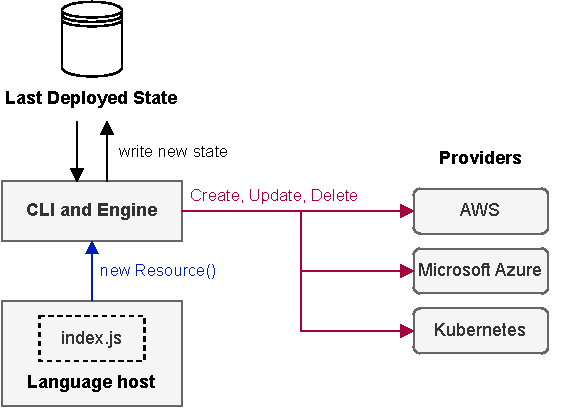
\includegraphics[width=.8\columnwidth]{analysis/pulumi_iac.pdf}
    \captionof{figure}{Overview of Pulumi deployment \cite{pulumi}}
    \label{fig:pulumi_iac}
    \endgroup
\end{center}

\subsection{Comparison}
Without even using the \acrshort{iac} tools, it is possible to identify a few differences. The tools integrated with the \gls{cloud} providers cannot be used outside their platform. The other two tools, Terraform and Pulumi, can be provisioned by different providers. One notable point concerns the syntax. Terraform and Microsoft Azure use descriptive syntaxes. These limit the variety of programming languages. Terraform has its own language which you need to familiarise yourself with the first time. \gls{aws} and Pulumi use imperative syntax, which leaves the choice of programming languages open.

Focusing on the practical side, other disparities were noted. These stem from a project that was carried out with the aim of comparing the different \acrshort{iac} tools mentioned in this section \ref{subsec:iac_tools} \cite{iac_tools}. Terraform has several advantages, including clear documentation, an understandable configuration language, real-time execution plans and the ability to structure the infrastructure by dividing scripts into separate files. Because \gls{cloud} providers have different services, it is impossible to reuse the same code with each of them. It is possible to maintain the overall architecture of the infrastructure if the entities are clearly separated in the scripts. On the Pulumi side, resources can be separated into classes or functions. Common code between providers is therefore limited to abstractions of classes and functions. Pulumi has developed a tool capable of converting Terraform scripts into Pulumi scripts. It differs from Terraform by using Pulumi \Gls{cloud} for infrastructure state management by default instead of a self-managed \acrshort{api}. This is an advantage of not needing to store state files locally and manage them. Terraform and Pulumi generally use \acrshort{api}s from \gls{cloud} providers to create resources. One case stands out with Pulumi, when it works with \gls{aws}, it uses the \gls{aws} \acrshort{sdk} service directly, which will create the resources. Concerning the \acrlong{a_arm} tool, it is less efficient than \gls{aws} \acrshort{cdk} because of the complexity of the configuration files. \gls{aws} \acrshort{cdk} offers better readability by being able to divide up the code as required. Despite all this, it should be noted that these four \acrshort{iac} tools were able to provision the project in question. \cite{iac_tools}


% ------------------------------------------------------------------------------
\section{\texorpdfstring{\gls{arm}}{} SystemReady}

% -- Your text goes here --
Manufacturer \gls{arm} has decided to introduce a certification programme called SystemReady \cite{systemready_program}. In 2020, as part of \gls{arm}'s Cassini project, SystemReady was introduced to address the compatibility concerns of users planning to move from x86 architectures to systems based on \gls{arm}'s processors \cite{systemready_approval}. \gls{arm} defines its programme as follows:
\begin{quote}
    \textit{\gls{arm} SystemReady is a compliance certification program based on a set of hardware and firmware standards: \acrfull{bsa} and \acrfull{bbr} specifications, plus a selection of supplements. This ensures that subsequent layers of software also ‘just work’. The compliance certification program tests and certifies that systems meet the SystemReady standards, giving confidence that operating systems \acrshort{os} and subsequent layers of software just work. \cite{systemready_program}}\\
\end{quote}

The \gls{arm} \acrshort{bsa} specification establishes a hardware basis for system software, including \acrshort{os}s, hypervisors and firmware, based on the 64-bit \gls{arm} architecture. This specification ensures that users can install, boot and run generic \acrshort{os}s and hypervisors \cite{bsa_standard}. The \acrshort{bbr} specification complements \acrshort{bsa} by defining the basic firmware requirements necessary to support any \acrshort{os} or hypervisor compatible with the \acrshort{bsa} specification \cite{bbr_standard}.

A number of advantages were mentioned in relation to the program \cite{systemready_program}:
\begin{itemize}
    \item[—] Compliance allows \acrshort{os}s and workloads to operate seamlessly on different \gls{arm} platforms.
    \item[—] Standardisation of a range of different devices and systems provides a stable basis and a choice of systems for all sectors.
    \item[—] Compliance with standards inspires confidence in software compatibility, so developers can concentrate on innovation and adding value to their products.
    \item[—] Compliance simplifies and accelerates time-to-market for partners.
    \item[—] Compliance makes it easy to identify \gls{arm}-based devices thanks to the "SystemReady certified" stamp.
    \item[—] Compliance makes it easy to deploy and maintain standard firmware interfaces, reducing maintenance costs.
    \item[—] Compliance reduces the costs associated with adopting a new platform by eliminating custom firmware engineering.
\end{itemize}

\subsection{SystemReady certifications}
To be able to adapt to different types of devices and markets, \gls{arm} has introduced four certifications. The first is SystemReady SR. It ensures the smooth operation of servers or workstations on a \gls{arm} chip. It is specially designed for Windows, Linux, VMware and \acrfull{bsd} environments. It targets generic out-of-the-box \acrshort{os}s and also supports legacy \acrshort{os}s on new devices. \cite{systemready_program}

SystemReady ES is designed to meet the needs of Windows, Linux, VMware and \acrshort{bsd} ecosystems based on \gls{arm} embedded systems. It also targets generic out-of-the-box \acrshort{os}s and supports legacy \acrshort{os}s on new devices. \cite{systemready_program}

SystemReady IR ensures that Linux and \acrshort{bsd} work perfectly on \gls{arm} embedded systems. It is ideally suited to the \acrshort{iot} sector. It mainly targets the Linux environment, but also custom images (Yocto, OpenWRT, buildroot) and pre-built images (Debian, Fedora, SUSE). \cite{systemready_program}

SystemReady LS specifies the correct operation of Linux \acrshort{os}s on \gls{arm} chips designed for servers. This certificate is mainly for hyperscalers. Hyperscalers are large \gls{cloud} service providers. \cite{systemready_program}

At present, a multitude of hardware design companies are partnering with \gls{arm} to follow the SystemReady standards. Several embedded systems are already certified and on the market.